\section{Einleitung}

Ziel der Arbeit im Rahmen der Vorlesung Robotik war es, das Spiel \glqq Vier Gewinnt\grqq ~auf einer LED-Matrix zu implementieren und eine Künstliche Intelligenz zu entwickeln, die es ermöglicht auch alleine das Spiel zu nutzen.

\section{Vier Gewinnt}
Bei \glqq Vier Gewinnt\grqq ~handelt es sich um ein Spiel, bei dem zwei Spieler auf einem klassischerweise 6x7 Feld (6 Zeilen, 7 Spalten) versuchen über das jeweilige Setzen von Steinen eine Reihe von vier Steinen zu erzeugen. Die Vorraussetzungen dabei sind, dass der jeweilige Stein am unteren Ende der Spalte gesetzt wird und die Spieler stets nacheinander am Zuge sind.

\begin{figure}[!hbt]
	\centering
	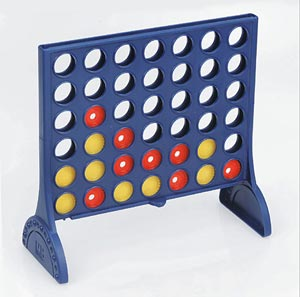
\includegraphics[scale=0.8]{4Gewinnt.jpeg}
	\caption{Ein klassisches Vier-Gewinnt-Spiel}
\end{figure}

Aus mathematischer Sicht ist \glqq Vier Gewinnt\grqq ~ein Spiel mit perfekter Information. Dies bedeutet, dass zu jedem Zeitpunkt alle vorhergehenden Züge bekannt sind. Diese perfekte Information sorgt dafür, dass das Spiel volständig gelöst ist. Daraus kann abgeleitet werden, dass der Ausgang des Spiels für zwei perfekt spielende Gegner davon abhängig ist, in welche Spalte der erste Stein gesetzt worden ist: Wurde der erste Stein in die mittlerste Spalte gesetzt, so gewinnt bei perfektem Spiel stets der erste Spieler. Beim Setzen in eine der Nachbarspalten, endet das Spiel unentschieden, sollte der erste Stein in eine der übrigen Spalten gesetzt werden, so gewinnt der zweite Spieler. 

\section{LED-Matrix}
Um \glqq Vier Gewinnt\grqq ~auf einer LED-Matrix abbilden zu können müssen zwei wesentliche Eigenschaften von der Matrix erfüllt werden: Zunächst muss die Matrix eine Mindestgröße von 6x7 besitzen, zum anderen muss sie fähig sein mindestens zwei unterschiedliche Farben abzubilden.
Bei der Suche nach einer geeigneten Matrix hat sich herausgestellt, dass vor allem die zweite Eigenschaft ein Problem darstellt.
Es konnte dennoch eine geeignete Matrix gefunden werden:
Das \glqq Adafruit 16x32 RGB LED matrix panel\grqq.

\begin{figure}[!hbt]
	\centering
	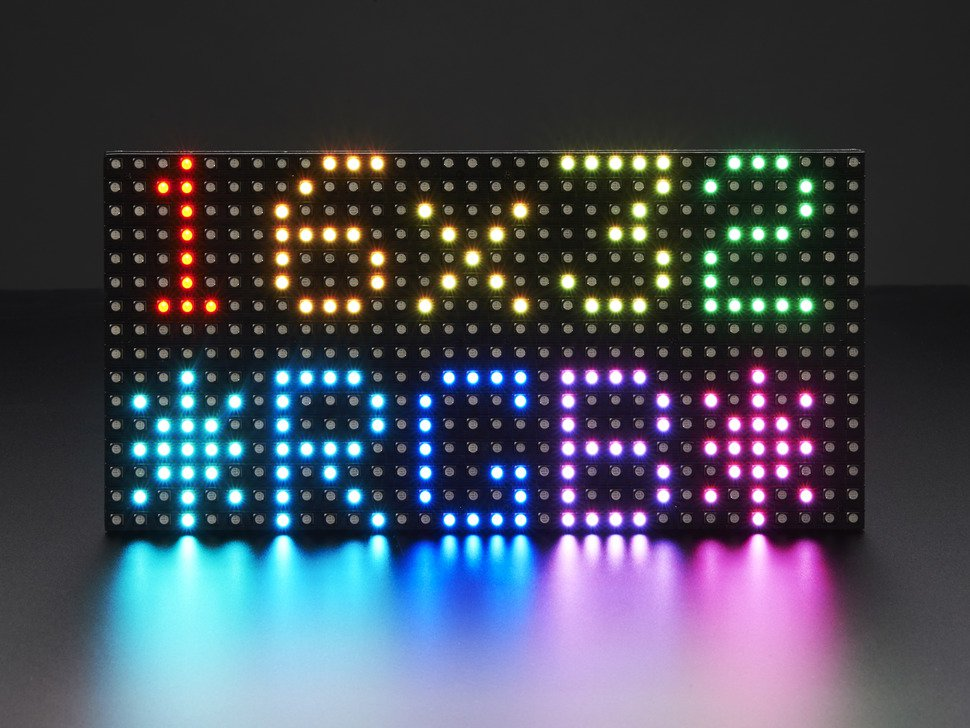
\includegraphics[scale=1]{RGBLEDMatrix.jpg}
	\caption{Verwendete LED-Matrix von Adafruit}
\end{figure}

Da die Matrix mit 16x32 deutlich über der Anforderung lag, wurde entschieden, dass auf der Matrix jeder Stein durch ein 2x2 Feld  dargestellt wird


\section{Ausblick}
